\section{Branches}

\subsection{RX-Line}
The RX Line model corresponds to a resistance in series with a inductance. The inductance is represented using resistive companion and therefore replaced by a resitance in parallel to a current source.

The user can define the RX Line in two ways. The first one is with the following parameters:

\begin{itemize}
\item name: Name of the component
\item node1: First node, where the resistance is connected
\item node2: Second node, where the inductance is connected
\item node3: Node between resistance and inductance 
\item resistance: Resistance in ohms
\item inductance: Inductance in H
\end{itemize}

\begin{figure}[h]
	\centering
	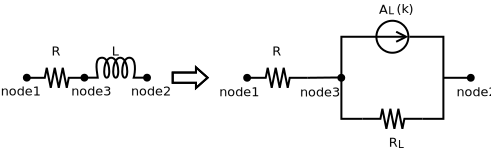
\includegraphics[scale=0.5]{img/RXLine} 
	\caption{RX Line model}
	\label{fig:RxLine}
\end{figure}

In this case, the function "applySystemMatrixStamp" will stamp the resistances $R$ between node1 and node3 and $R_L$ between node3 and node2 to the conductance matrix $G$. The function "step" will recalculate the value of $A_L$ as in equation \ref{eq:AL} and stamp it between node3 and node2 to the vector $A$. The function "poststep" will update the values of inductor current and voltage using equations \ref{eq:inductorCurrent} and \ref{eq:inductorVoltage}.

\begin{align}
\begin{split}
&
\begin{matrix}
& \cdots & node1 & node2 &  node3 & \cdots
\end{matrix}\\[-6pt]
G \quad = \quad
\begin{matrix}
\vdots\\[8pt]
node1\\[8pt]
node2\\[8pt]
node3\\[8pt]
\vdots\\
\end{matrix}
&
\begin{bmatrix}
	\quad & \quad &  \\[8pt]
	\quad & \quad \dfrac{1}{R} & \quad & \quad \dfrac{-1}{R} & \quad  \\[8pt]
	\quad & \quad & \quad \dfrac{1}{R_L} & \quad \dfrac{-1}{R_L} & \quad \\[8pt]
	\quad & \quad \dfrac{-1}{R} & \quad \dfrac{-1}{R_L} & \dfrac{1}{R}+\dfrac{1}{R_L} & \quad\\[8pt]
	\quad\\ 
\end{bmatrix}
\end{split}
\end{align}
\begin{align}
\begin{split}
A\quad = \quad
\begin{matrix}
\vdots\\[8pt]
node1\\[8pt]
node2\\[8pt]
node3\\[8pt]
\vdots\\
\end{matrix}
\begin{bmatrix}
	\quad \\[8pt]
	\quad \\[8pt]
	A_L(k) \\[8pt]
	-A_L(k) \\[8pt]
	\quad
\end{bmatrix}
\end{split}
\end{align}

The second way of define the RX Line is defining only two nodes (node1 and node2). In this case, the equivalent circuit in figure \ref{fig:RxLine2} is considered.

\begin{figure}[ht]
	\centering
	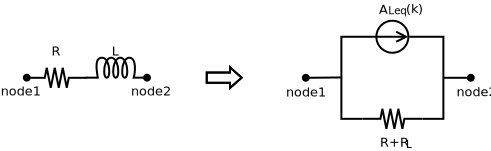
\includegraphics[scale=0.5]{img/RXLine2} 
	\caption{RX Line model with two nodes}
	\label{fig:RxLine2}
\end{figure}

The function "applySystemMatrixStamp" will stamp the resistance $R+R_L$ between node1 and node2 to the conductance matrix $G$.

\begin{align}
\begin{split}
&
\begin{matrix}
& \cdots & node1 & \quad node2 & \cdots
\end{matrix}\\[-5pt]
G \quad = \quad
\begin{matrix}
\vdots\\[6pt]
node1\\[6pt]
node2\\[6pt]
\vdots\\
\end{matrix}
&
\begin{bmatrix}
	\quad & \quad &  \\[6pt]
	\quad & \dfrac{1}{R+R_L} & \dfrac{-1}{R+R_L} & \quad  \\[6pt]
	\quad & \dfrac{-1}{R+R_L} & \dfrac{1}{R+R_L} & \quad \\[6pt]
	\quad &  & 
\end{bmatrix}
\end{split}
\end{align}

The function "step" will update the values of $A_L$ as in equation \ref{eq:AL} and $A_{Leq}(k)$. $A_{Leq}$ will be stamped to the vector $A$ as in equation \ref{eq:AleqStamp}.

\begin{equation}
A_{Leq}(k)=A_L(k) \cdot \frac{R_L}{R_L+R}
\end{equation}

\begin{align} \label{eq:AleqStamp}
\begin{split}
A\quad = \quad
\begin{matrix}
\vdots\\[8pt]
node1\\[8pt]
node2\\[8pt]
\vdots\\
\end{matrix}
\begin{bmatrix}
	\quad \\[8pt]
	-A_{Leq}(k) \\[8pt]
	A_{Leq}(k) \\[8pt]
	\quad
\end{bmatrix}
\end{split}
\end{align}

The function "poststep" will calculate the values of the line voltage and current and inductor voltage and current for the actual step (k+1).

\begin{equation}
	v_{Line}(k+1) = v_{node1}(k+1) - v_{node2}(k+1) 
\end{equation}

\begin{equation}
	i_{Line}(k+1) = \frac{v_{Line}(k+1)}{R+R_L} + A_{Leq} 
\end{equation}

\begin{equation}
	v_L(k+1) = v_{Line}(k+1) - R \cdot i_{Line}(k+1)
\end{equation}

\begin{equation}
	i_L(k+1) = i_{Line}(k+1)
\end{equation}

In both cases, the function "init" is setting every initial value to zero.

\subsection{PI-Line}
The Pi Line model corresponds to a resistance in series with a inductance and two shunt capacitors as shown in figure \ref{fig:PiLine}. The inductance and the capacitance are represented using resistive companion and therefore replaced by a resitance in parallel to a current source.

The following parameters are defined by the user:

\begin{itemize}
\item name: Name of the component
\item node1: First node, where the resistance and the first capacitor are connected
\item node2: Second node, where the inductance and the second capacitor are connected
\item node3: Node between resistance and inductance 
\item resistance: Resistance in ohms
\item inductance: Inductance in H
\item capacitance: Capacitance in F
\end{itemize}

\begin{figure}[h]
	\centering
	\includegraphics[scale=0.5]{img/PiLine} 
	\caption{Pi Line model}
	\label{fig:PiLine}
\end{figure}

The function "init" will initialize all currents and voltages with zero.

The function "applySystemMatrixStamp" will stamp the resistances $R$ between node1 and node3, $R_L$ between node3 and node2, $R_{C1}$ between node1 and reference node and $R_{C2}$ between node2 and reference node to the conductance matrix $G$.

The function "step" will recalculate the value of $A_L$, $A_{C1}$ and $A_{C2}$ and stamp it to the vector $A$.

The function "poststep" will update the values of inductor and capacitors current and voltage.

\begin{align}
\begin{split}
&
\begin{matrix}
& \quad \cdots & \quad node1 \quad & \quad node2 \quad &  \quad node3 & \cdots
\end{matrix}\\[-6pt]
G \quad = \quad
\begin{matrix}
\vdots\\[8pt]
node1\\[8pt]
node2\\[8pt]
node3\\[8pt]
\vdots\\
\end{matrix}
&
\begin{bmatrix}
	\quad & \quad &  \\[8pt]
	\quad & \quad \dfrac{1}{R} + \dfrac{1}{R_{C1}} & \quad & \quad \dfrac{-1}{R} & \quad  \\[8pt]
	\quad & \quad & \quad \dfrac{1}{R_L} + \dfrac{1}{R_{C2}} & \quad \dfrac{-1}{R_L} & \quad \\[8pt]
	\quad & \quad \dfrac{-1}{R} & \quad \dfrac{-1}{R_L} & \dfrac{1}{R}+\dfrac{1}{R_L} & \quad\\[8pt]
	\quad\\ 
\end{bmatrix}
\end{split}
\end{align}
\begin{align}
\begin{split}
A\quad = \quad
\begin{matrix}
\vdots\\[8pt]
node1\\[8pt]
node2\\[8pt]
node3\\[8pt]
\vdots\\
\end{matrix}
\begin{bmatrix}
	\quad \\[8pt]
	A_{C1}(k) \\[8pt]
	A_L(k) + A_{C2}(k) \\[8pt]
	-A_L(k) \\[8pt]
	\quad
\end{bmatrix}
\end{split}
\end{align}

\subsection{Transformer}
\subsubsection{Typical Parameters}

\begin{equation}
	Z = u_{kr} \cdot \frac{U_{r1}^2}{S_{r}}
\end{equation}

\begin{equation}
	R = u_{Rr} \cdot \frac{U_{r1}^2}{S_{r}}
\end{equation}

\begin{equation}
	X = \sqrt{Z^2-R^2}
\end{equation}

\begin{equation}
	R_{Fe} = \frac{U_{r1}^2}{P_{Fe}}
\end{equation}

\begin{equation}
	X_{0} = \frac{U_{r1}}{\sqrt{3} I_{0}}
\end{equation}

\subsubsection{Nodal Analysis Representation}

The ideal transformer has an inner node which requires an extension of the system matrix. $j$ is the high voltage node while $k$ is the low voltage node. $l$ is the inner node of the transformer. The transformer ration is defined as $T=V_{j}/V_{k}$. A phase shift can be introduced if $T$ is considered as complex number.
\begin{align}
	& \begin{matrix}
	&  j & \quad k & \quad l\\
	\end{matrix}\\
	\begin{matrix}
	j\\
	k\\
  l\\
	\end{matrix}
	& \begin{bmatrix}
	\quad & \quad & -1\\
	& & T\\
	1 & -T & 0\\
	\end{bmatrix}
	\begin{bmatrix}
	v_j\\
	v_k\\
	i_{l}\\
	\end{bmatrix}
	=
	\begin{bmatrix}
	\\
	\\
	0\\
	\end{bmatrix}	
\end{align}
